\section{Definitions File \& Custom File Processing}\label{definitions-file-custom-file-processing}

\subsection{Description of ``Def'' input file}\label{description-of-def-input-file}

Some of the data formats have inherent omissions (e.g.~TMY does not have location data, BLAST ASCII does not have elevations). In order to overcome this limitation and to provide further flexibility, a definitions file (extension must be .def) is implemented. By naming this with the same ``file name'' as your input file (in the same folder), the weather converter will read the format and use that data, as appropriate, in the file conversions. The .def file uses Fortran ``Namelist'' input fields as shown in the example below. For flexibility, you can also define a ``presets.def'' file (such as when you have a list of files to process and the format or some portion is all the same between the group of files. The two def files (one named the same as the file name for the raw data and one named presets.def) will both be processed. Conflicts between the two will be shown in the .audit file. The set of namelist groups is:

\begin{itemize}
\item
  \&location - Location data
\item
  \&miscdata - Comments to be applied to ``COMMENT2'' in the EPW file and ``Source Data''
\item
  \&wthdata - weather data specifications including file type, custom formats
\item
  \&datacontrol - user specified control over ``missing'' data (Custom format only)
\end{itemize}

\textbf{Note that the ``Def'' formats are entirely different from the usual IDF formats of EnergyPlus. No commas separate fields. No semicolon terminates the entry.}

\begin{lstlisting}
&location
City = 'Hong Kong'
StateProv = ' '
Country = 'CHN'
InLat = 22.75
InLong = 115
InTime = 8
InElev = 0
InWMO = 450040
/
\end{lstlisting}

\begin{lstlisting}
&miscdata
Comments1 = 'This file was given to us by....'
SourceData = 'Original xyz data'
/
\end{lstlisting}

The ``slash'' (/) character terminating each block is very important - omissions results in incorrect reading of data.

Definitions File Details are shown in the following table. You may leave out a field if you wish - the program will use whatever default is applicable (or usable) from the data format. All data formats accept this additional file. Only Custom format currently uses the \&datacontrol element. And only Custom format input type uses the Data Elements, Format and Conversion factors from the \&wthdata element.

Note that strings in the ``def'' should be enclosed in single quotes if there is more than one word in the string - if only one word, quotes do not need to be used.

% table 4
\begin{longtable}[c]{p{2.12in}p{1.5in}p{2.37in}}
\caption{Definitions File \&location description \label{table:definitions-file-location-description}} \tabularnewline
\toprule 
\& location Field Description & Field Name & Type \tabularnewline
\midrule
\endfirsthead

\caption[]{Definitions File \&location description} \tabularnewline
\toprule 
\& location Field Description & Field Name & Type \tabularnewline
\midrule
\endhead

Name of City & City & String \tabularnewline
State or Province & StateProv & String \tabularnewline
Country Code & Country & String (3 characters) \tabularnewline
Latitude (N+/S-) & InLat & Numeric \tabularnewline
Longitude (W-/E+) & InLong & Numeric \tabularnewline
Time Zone (GMT +/-) & InTime & Numeric \tabularnewline
Elevation (meters) & InElev & Numeric \tabularnewline
WMO \# & InWMO & Numeric or String (6 characters) \tabularnewline
\bottomrule
\end{longtable}

\subsection{Expected Formats for \&location}\label{expected-formats-for-location}

\subsubsection{Fields: City, StateProv, Country}\label{fields-city-stateprov-country}

These fields are string variables. If Country is \emph{not} included, an attempt to use the State/Prov entry may be used to determine country. Otherwise, these fields are not validated and are used to create part of the ``location'' header record in the EPW file. City can be up to 30 characters in length; StateProv up to 15 characters; Country up to 10 characters (standard 3 character abbreviation preferred).

\subsubsection{Fields: InLat, InLong}\label{fields-inlat-inlong}

These fields are decimal equivalent for Latitude and Longitude. The convention is North Latitude is positive; South is negative. Likewise, East Longitude is positive; West Longitude is negative. That is, if your latitude is N 30° 15' (North 30 degrees, 15 minutes) then your input is +30.25.

\subsubsection{Field: InTime}\label{field-intime}

This field is the decimal equivalent for the Time Zone value. The convention is GMT +/-. That is, if your time zone is ``behind'' GMT time by 6 hours, your input would be -6.

\subsubsection{Field: InElev}\label{field-inelev}

This field is the location elevation in meters. Range can be from -300 to 6096. (These are the values from EnergyPlus - there is no validation of these in the weather converter.)

\subsubsection{Field: InWMO}\label{field-inwmo}

This field is the WMO (World Meterological Organization) number for the location. Though not validated per se, if found in the ``design conditions'' auxiliary files, the Design Day information can be generated.

% table 5
\begin{longtable}[c]{@{}lll@{}}
\caption{Definitions File - \&miscdata description \label{table:definitions-file-miscdata-description}} \tabularnewline
\toprule 
\& miscdata Field Description & Field Name & Type \tabularnewline
\midrule
\endfirsthead

\caption[]{Definitions File - \&miscdata description} \tabularnewline
\toprule 
\& mischata Field Description & Field Name & Type \tabularnewline
\midrule
\endhead

String for Comments 1 header & Comments1 & String \tabularnewline
String for Comments 2 header & Comments2 & String \tabularnewline
String for Source Data in Location header & SourceData & String \tabularnewline
URL for output & OutputURL & String \tabularnewline
\bottomrule
\end{longtable}

\subsection{Expected Formats for \&miscdata}\label{expected-formats-for-miscdata}

\subsubsection{Fields: Comments1, Comments2}\label{fields-comments1-comments2}

These are strings. After concatenation, they become part of the comment header lines in the EPW headers. Up to 150 characters each is allowed.

\subsubsection{Field: SourceData}\label{field-sourcedata}

This string is applied to the ``Source Data'' field in the Location Header. Up to 60 characters is allowed.

\subsubsection{Field: OutputURL}\label{field-outputurl}

When a list of files is being processed, one of the outputs that results from the processing is a KML (Keyhole Markup Language) file that can be used with Google Earth to pinpoint the locations of the weather site. This field can be used to set this URL for later output. The list file format also includes a URL as its third (optional) parameter. If included, this input would overwrite other URL designations.

% table 6
\begin{longtable}[c]{p{2.71in}p{1.5in}p{1.79in}}
\caption{Definitions file - \&wthdata description \label{table:definitions-file-wthdata-description}} \tabularnewline
\toprule 
\& wthdata Field Description & Field Name & Type \tabularnewline
\midrule
\endfirsthead

\caption[]{Definitions file - \&wthdata description} \tabularnewline
\toprule 
\& wthdata Field Description & Field Name & Type \tabularnewline
\midrule
\endhead

Input File Type & InputFileType & String \tabularnewline
Number of records per hour & NumInHour & Integer \tabularnewline
Data Element Names & DataElements & Strings \tabularnewline
Data Units & DataUnits & Strings \tabularnewline
Multiplicative Conversion Factors for Data & DataConversionFactors & Numeric \tabularnewline
Special Missing Values & DataMissingValues & Numeric \tabularnewline
Format for input & InFormat & Format String or "delimited" \tabularnewline
Delimiter Character & DelimiterChar &  \tabularnewline
Decimal Delimiter Character & DecimalSymbolChar & String \tabularnewline
Date Separator & DateSeparator & String (single character) \tabularnewline
\bottomrule
\end{longtable}

\subsection{Expected Formats for \&wthdata}\label{expected-formats-for-wthdata}

\subsubsection{Field: InputFileType}\label{field-inputfiletype}

You can always use this field and def file to ``override'' the default input format type that depends on the extension of your file (see Table~\ref{table:input-file-extensions-with-implied-data-types}. Input File Extensions with implied Data types). A complete set of valid values for Input File types is shown in the following table. Data Files are described more fully in the section Source Weather Data Formats that occurs later in this document.

% table 7
\begin{longtable}[c]{@{}ll@{}}
\caption{Input File Type Values \label{table:input-file-type-values}} \tabularnewline
\toprule 
Value & File Type Description \tabularnewline
\midrule
\endfirsthead

\caption[]{Input File Type Values} \tabularnewline
\toprule 
Value & File Type Description \tabularnewline
\midrule
\endhead

Tmy or tm2 & TMY2 Data File \tabularnewline
Iwec or iwc & IWEC Data File \tabularnewline
Samson or dat & SAMSON Data File \tabularnewline
wyec2 or wy2 & WYEC2 Data File \tabularnewline
Fmt or txt & DOE-2 FMT File \tabularnewline
Clm or esp-r & ESP-r Formatted (CLM) data file \tabularnewline
Blast or asc & BLAST ASCII Data File \tabularnewline
Tmy & TMY Data File \tabularnewline
Epw & EPW Data File \tabularnewline
Csv & EPW - CSV Data File \tabularnewline
Wea & Ecotect wea Data File \tabularnewline
Swera or swe & SWERA Data File \tabularnewline
Custom or User & Custom Data File \tabularnewline
\bottomrule
\end{longtable}

\subsubsection{Field: NumInHour}\label{field-numinhour}

This field can be used to specify multi-interval (per hour) files. Without this field, the only formats that can have multiple intervals per hour are the EPW and CSV file formats - using the header record DataPeriods value for that field.

\subsubsection{Fields below only used in ``Custom'' format processing}\label{fields-below-only-used-in-custom-format-processing}

\subsubsection{Field: DataElements}\label{field-dataelements}

For custom files, you will need to indicate which data elements are in which positions of the raw data file. The fields must come from a standardized list of names see following tables that include internal names (short and long - as shown in Table 8) as well as the EnergyPlus CSV format names (short and long - shown in Table~\ref{table:names-from-the-energyplus-csv-files}) plus some further elements that can be specified when the standard data elements are not part of the raw data (as shown in Table~\ref{table:auxiliary-data-for-custom-files}). ``Ignore'' is used to skip a raw data field that is not applicable to the weather converter formats. Note that variables listed in the following table (in italics) are allowed for flexibility - i.e.~wetbulb temperature can be used to determine relative humidity and/or dewpoint temperature. The following three tables illustrate the names for data elements.

\begin{longtable}[c]{p{1.5in}p{2.5in}p{1.0in}p{1.0in}}

\caption{Internal Data Element Names (directly applicable to EPW) \label{table:internal-data-element-names-directly}} \tabularnewline
\toprule 
Short Name & Long Name & Default EPW Units & Used by EnergyPlus \tabularnewline
\midrule
\endfirsthead

\caption[]{Internal Data Element Names (directly applicable to EPW)} \tabularnewline
\toprule
Short Name & Long Name & Default EPW Units & Used by EnergyPlus \tabularnewline
\midrule
\endhead

year & Year & - & N \tabularnewline
month & Month & - & Y \tabularnewline
day & Day & - & Y \tabularnewline
hour & hour & - & Y \tabularnewline
minute & minute & - & N \tabularnewline
datasource & datasource & - & N \tabularnewline
drybulb & dry\_bulb\_temperature & \si{\celsius} & Y \tabularnewline
dewpoint & dew\_point\_temperature & \si{\celsius} & Y \tabularnewline
relhum & relative\_humidity & \si{\percent} & Y \tabularnewline
atmos\_pressure & atmospheric\_pressure & \si{\pascal} & Y \tabularnewline
exthorrad & extraterrestrial\_horizontal\linebreak\_radiation & \si{\watt\hour\per\meter\squared} & N \tabularnewline
extdirrad & extraterrestrial\_direct\linebreak\_normal\_radiation & \si{\watt\hour\per\meter\squared} & N \tabularnewline
horirsky & horizontal\_infrared\linebreak\_radiation\_intensity\_from\_sky & \si{\watt\hour\per\meter\squared} & Y \tabularnewline
glohorrad & global\_horizontal\_radiation & \si{\watt\hour\per\meter\squared} & N \tabularnewline
dirnorrad & direct\_normal\_radiation & \si{\watt\hour\per\meter\squared} & Y \tabularnewline
difhorrad & diffuse\_horizontal\_radiation & \si{\watt\hour\per\meter\squared} & Y \tabularnewline
glohorillum & global\_horizontal\_illuminance & \si{\lux} & N \tabularnewline
dirnorillum & direct\_normal\_illuminance & \si{\lux} & N \tabularnewline
difhorillum & diffuse\_horizontal\_illuminance & \si{\lux} & N \tabularnewline
zenlum & zenith\_luminance & \si{\lux} & N \tabularnewline
winddir & wind\_direction & \si{\degree} & Y \tabularnewline
windspd & wind\_speed & \si{\m/s} & Y \tabularnewline
totskycvr & total\_sky\_cover & tenths & N \tabularnewline
opaqskycvr & opaque\_sky\_cover & tenths & N \tabularnewline
visibility & visibility & \si{\km} & N \tabularnewline
ceiling\_hgt & ceiling\_height & \si{\m} & N \tabularnewline
presweathobs & present\_weather\_observation & - & Y \tabularnewline
presweathcodes & present\_weather\_codes & - & Y \tabularnewline
precip\_wtr & precipitable\_water & \si{\mm} & N \tabularnewline
aerosol\_opt\_depth & aerosol\_optical\_depth & thousandths & N \tabularnewline
snowdepth & snow\_depth & \si{\cm} & Y \tabularnewline
days\_last\_snow & days\_since\_last\_snow & - & N \tabularnewline
Albedo & albedo & - & N \tabularnewline
liq\_precip\_depth & liquid\_precip\_depth & \si{\mm} & Y \tabularnewline
liq\_precip\_rate & liquid\_precip\_rate & \si{\hour} & N \tabularnewline
\bottomrule
\end{longtable}

The following table illustrates that the EnergyPlus CSV header names can be used for data elements in DEF files, if desired.

% table 9
\begin{longtable}[c]{p{1.5in}p{1.5in}p{1.5in}p{1.5in}}
\caption{Names from the EnergyPlus CSV files \label{table:names-from-the-energyplus-csv-files}} \tabularnewline
\toprule 
Short Name & Long Name & Default EPW Units & Used by EnergyPlus \tabularnewline
\midrule
\endfirsthead

\caption[]{Names from the EnergyPlus CSV files} \tabularnewline
\toprule 
Short Name & Long Name & Default EPW Units & Used by EnergyPlus \tabularnewline
\midrule
\endhead

Date & Date (used to derive Month/Day) & - & N \tabularnewline
hh:mm & HH:MM (used to derive hour/minute) & - & N \tabularnewline
datasource & datasource & - & N \tabularnewline
Drybulb & dry bulb temperature & \si{\celsius} & Y \tabularnewline
dewpoint & dew point temperature & \si{\celsius} & Y \tabularnewline
Relhum & relative humidity & \% & Y \tabularnewline
atmos pressure & atmospheric pressure & Pa & Y \tabularnewline
exthorzrad & extraterrestrial horizontal radiation & \si{\watt\hour\per\meter\squared} & N \tabularnewline
extdirrad & extraterrestrial direct normal radiation & \si{\watt\hour\per\meter\squared} & N \tabularnewline
horzirsky & horizontal infrared radiation intensity from sky & \si{\watt\hour\per\meter\squared} & Y \tabularnewline
glohorzrad & global horizontal radiation & \si{\watt\hour\per\meter\squared} & N \tabularnewline
dirnorzrad & direct normal radiation & \si{\watt\hour\per\meter\squared} & Y \tabularnewline
difhorzrad & diffuse horizontal radiation & \si{\watt\hour\per\meter\squared} & Y \tabularnewline
glohorzillum & global horizontal illuminance & \si{\lux} & N \tabularnewline
dirnorzillum & direct normal illuminance & \si{\lux} & N \tabularnewline
difhorzillum & diffuse horizontal illuminance & \si{\lux} & N \tabularnewline
Zenlum & zenith luminance & \si{\lux} & N \tabularnewline
winddir & wind direction & \si{\degree} & Y \tabularnewline
windspd & wind speed & \si{m/s} & Y \tabularnewline
totskycvr & total sky cover & tenths & N \tabularnewline
opaqskycvr & opaque sky cover & tenths & N \tabularnewline
visibility & visibility & \si{\km} & N \tabularnewline
ceiling hgt & ceiling height & \si{\m} & N \tabularnewline
presweathobs & present weather observation & - & Y \tabularnewline
presweathcodes & present weather codes & - & Y \tabularnewline
precip wtr & precipitable water & \si{\mm} & N \tabularnewline
aerosol opt depth & aerosol optical depth & thousandths & N \tabularnewline
snowdepth & snow depth & \si{\cm} & Y \tabularnewline
days last snow & days since last snow & - & N \tabularnewline
Albedo & albedo & - & N \tabularnewline
rain & liquid precipitation depth & \si{\mm} & Y \tabularnewline
rain quantity & liquid precipitation rate & \si{\hour} & N \tabularnewline
\bottomrule
\end{longtable}

\subsection{Custom Files - Auxiliary Data}\label{custom-files---auxiliary-data}

Often raw data files will not have the preceding elements but similar elements that can be used to derive the values used in the EPW files and in EnergyPlus. (For example, dew point temperature and relative humidity are needed and can be derived from dry builb temperature and a humidity indicating element such as wet bulb temperature or humidity ratio). The following table contains the data element names that can be used in the Weather Converter program to derive other data which will then be placed into the EPW data fields.

% table 10
\begin{longtable}[c]{p{1.5in}p{1.5in}p{1.5in}p{1.5in}}
\caption{Auxiliary Data for Custom Files \label{table:auxiliary-data-for-custom-files}} \tabularnewline
\toprule 
Short Name & Long Name & Units & Used by EnergyPlus \tabularnewline
\midrule
\endfirsthead

\caption[]{Auxiliary Data for Custom Files} \tabularnewline
\toprule 
Short Name & Long Name & Units & Used by EnergyPlus \tabularnewline
\midrule
\endhead

wetbulb & wet\_bulb\linebreak\_temperature & \si{\celsius} & N \tabularnewline
humratio & humidity\_ratio & \si{\g/kg} & N \tabularnewline
dirhorrad & direct\_horizontal\linebreak\_radiation & \si{\watt\hour\per\meter\squared} & N \tabularnewline
interval & Interval & unit & N \tabularnewline
hour\_yr & hour\_of\_year &\si{\hour} & N \tabularnewline
time & Time & hh:mm & N \tabularnewline
hh:mm & HH:MM & hh:mm & N \tabularnewline
Date & Date & mm/dd/yyyy & N \tabularnewline
\bottomrule
\end{longtable}

Explanation of these data elements follows:

\subsubsection{Wetbulb (Wet Bulb Temperature)}\label{wetbulb-wet-bulb-temperature}

If you have the wet bulb temperature, this data element can be used to derive the dew point temperature and relative humidity.

\subsubsection{HumRatio (Humidity Ratio)}\label{humratio-humidity-ratio}

If you have the humidity ratio, this data element can be used to derive the dew point temperature and relative humidity.

\subsubsection{Dirhorrad (Direct Horizontal Radiation)}\label{dirhorrad-direct-horizontal-radiation}

If you have direct horizontal radiation (and at least one other solar element from global horizontal radiation or diffuse horizontal radaition), this data element will be used to derive the direct normal radiation.

\subsubsection{Interval}\label{interval}

If your ``number of records per hour'' is \textgreater{}1, then you can designate each interval of that hour with this field.

\subsubsection{Hour\_Of\_Year}\label{hourux5fofux5fyear}

If you wish, you can just put in the hour of the year for each record. Note that if no date element is entered, then the default is that the data is in hour of the year (including possible number of records per hour).

\subsubsection{Time (or HH:MM)}\label{time-or-hhmm}

Time can be entered (rather than hour) and the units must be hh:mm; this is then decoded on each record to the appropriate hour.

\subsubsection{Date}\label{date}

Dates can be entered as month, day, and year. The units field must be entered and should designate the format for the date decoding. Date separator characters for this field are entered in the DateSeparator item. Default date separator is ``/'' and that is what is used in the table that shows the allowable units:

% table 11
\begin{longtable}[c]{@{}lll@{}}
\caption{Allowable date formats for Custom Data entries. \label{table:allowable-date-formats-for-custom-data}} \tabularnewline
\toprule 
Units Format & Interpretation & Example \tabularnewline
\midrule
\endfirsthead

\caption[]{Allowable date formats for Custom Data entries.} \tabularnewline
\toprule 
Units Format & Interpretation & Example \tabularnewline
\midrule
\endhead

mm/dd/yyyy mm/dd/yy m/d/y & Month, day, year & 12/13/2009 \tabularnewline
yyyy/mm/dd yy/mm/dd y/m/d & Year, month, day & 2009/12/13 \tabularnewline
dd/mm/yyyy dd/mm/yy d/m/y & Day, month, year & 13/12/2009 \tabularnewline
\bottomrule
\end{longtable}

\subsubsection{Field: DataUnits}\label{field-dataunits}

There should be as many DataUnits entries as DataElement entries. These are not generally used but may be used in the future for automatic conversions. The exception to this is ``temperature'' fields. Use ``f'' for Fahrenheit, ``k'' for Kelvin temperatures. Note that the DataConversionFactor for this field will be applied prior to conversion. (Many formats use integer numbers to represent values that are in tenths, for example.)

\subsubsection{Field: DataConversionFactors}\label{field-dataconversionfactors}

There should be as many DataConversionFactors entries as DataElement entries. These factors are multiplicative factors (i.e.~the input value is multiplied by this factor) and can be used to process input data into the values used in the EPW weather files.

\subsubsection{Field: DataMissingValues}\label{field-datamissingvalues}

There should be as many entries (though some can be blank) as DataElement entries. The values entered will override the default ``missing'' values (from the EPW data dictionary) and, whereas the defaults may be interpreted as a \textgreater{} = missing value (i.e. \textgreater{} = 999), these values will be exact (i.e. = -999.)

\subsubsection{Field: InFormat}\label{field-informat}

The value in this field should be ``delimited'' if you are using a free format data file or specify a ``Fortran style'' format statement.

\subsubsection{Field: DelimiterChar}\label{field-delimiterchar}

If you use a ``delimited'' format file, you need to specify a delimiter character. Only a single character may be specified.

\subsubsection{Field: DecimalSymbolChar}\label{field-decimalsymbolchar}

A single character can be used to specify the decimal ``point'' character. Default is the US Standard ``.''. With use of DelimiterChar and this field, one can essentially use the fields to specify European Standard Excel export formats.

\subsubsection{Field: DateSeparator}\label{field-dateseparator}

If you are entering the aforementiond ``date'' Data Element and your date separator is a character other than slash (``/''), then you need to enter a single character so the program can interpret your date entries.

% table 12
\begin{longtable}[c]{p{1.81in}p{1.65in}p{2.52in}}
\caption{Definitions file - \&datacontrol description \label{table:definitions-file-datacontrol-description}} \tabularnewline
\toprule 
\& datacontrol Field Description & Field Name & Type \tabularnewline
\midrule
\endfirsthead

\caption[]{Definitions file - \&datacontrol description} \tabularnewline
\toprule 
\& datacontrol Field Description & Field Name & Type \tabularnewline
\midrule
\endhead

Records to Skip & NumRecordsToSkip & Integer \tabularnewline
Records to Read & MaxNumRecordsToRead & Integer \tabularnewline
Missing Data Action & MissingDataAction &  \tabularnewline
Missing Wind Direction Action & MissingWindDirAction &  \tabularnewline
Missing Wind Direction Value & MissingWindDirValue & Real \tabularnewline
Missing Opaque Sky Cover Action & MissingOpaqueSky\linebreak
CoverAction &  \tabularnewline
Missing Opaque Sky Cover Value & MissingOpaqueSky\linebreak
CoverValue & Real (Value 0.0 to 10.0) - tenths of sky cover \tabularnewline
Maximum Wind Speed & MaxWindSpeed & Real \tabularnewline
Maximum Direct Solar & MaxDirectSolar & Real \tabularnewline
Maximum Diffuse Solar & MaxDiffuseSolar & Real \tabularnewline
Maximum Illuminance Value & MaxIlluminanceValue & Real \tabularnewline
Generate Solar Radiation Warnings & GenerateSolarRadiationWarnings &  \tabularnewline
Generate Illuminance Warnings & GenerateIlluminanceWarnings &  \tabularnewline
\bottomrule
\end{longtable}

\subsection{Expected Formats for \&datacontrol}\label{expected-formats-for-datacontrol}

Most of the items in this element are particularly applicable to custom format input files. Currently, they are only used in custom files, but may be more generally applicable in future releases.

\subsubsection{Field: NumRecordsToSkip}\label{field-numrecordstoskip}

This is an integer number of records to skip during processing. You might use this if your input file has some information at the top of the file.

\subsubsection{Field: MaxNumRecordsToRead}\label{field-maxnumrecordstoread}

This is an integer number of records to read (typically 8760 for a full year). You might use this if your input file has some information after the data records.

\subsubsection{Fields: MissingDataAction, MissingWindDirAction, MissingOpaqueSkyCoverAction}\label{fields-missingdataaction-missingwinddiraction-missingopaqueskycoveraction}

These fields tell the converter program what to do with ``missing'' data. Missing data can be found in two forms: totally not included in the DataElements or a missing value (as defined in the EPW format). Valid values for these fields are:

\begin{itemize}
\item
  DEFAULT - use the default processing that the weather converter already uses - starts off with a specific value and updates if data is found.
\item
  CONSTANT - use a constant value to replace all missing data
\item
  RANDOM - use a random number to generate the missing data
\end{itemize}

An additional value for MissingOpaqueSkyCoverAction is:

\begin{itemize}
\tightlist
\item
  TOTALSKY - use the value for Total Sky Cover
\end{itemize}

\subsubsection{Fields: MissingWindDirValue, MissingOpaqueSkyCoverValue}\label{fields-missingwinddirvalue-missingopaqueskycovervalue}

The values specified in this field are used with the action fields previously mentioned.

\subsubsection{Field: MaxWindSpeed}\label{field-maxwindspeed}

The default maximum wind speed (40m/s) may not be enough for some locations - this allows the override capability.

\subsubsection{Field: MaxDirectSolar, MaxDiffuseSolar, MaxIlluminanceValue}\label{field-maxdirectsolar-maxdiffusesolar-maxilluminancevalue}

Default maximum solar values may not be enough for some locations - this allows the override capability.

\subsubsection{Field: GenerateSolarRadiationWarnings, GenerateIlluminanceWarnings}\label{field-generatesolarradiationwarnings-generateilluminancewarnings}

If you don't want to see extra warnings when input values are greater than max values (default or as specified in previous fields), use NO as the keyword. Use YES to make sure you see the warnings. Default is YES.

\subsection{Def File Examples}\label{def-file-examples}

In the following examples, every attempt has been made to make sure that these work with the Weather Converter program. However, we cannot foresee all possible combinations. \textbf{Caveat emptor - user beware.}

Here's an example where the delimiter between fields is a semi-colon (;) and the decimal symbol character is a comma (,) - typical of some non-USA regional settings:

\begin{lstlisting}
&location
City = <cityname>
StateProv = <state/province>
Country = <country>
InWMO = <wmo>
InLat = <latitude>
InLong = <longitude>
InElev = <elevation>
InTime = <timezone>
/
\end{lstlisting}

\begin{lstlisting}
&wthdata
NumInHour = 1
InputFileType = 'CUSTOM'
InFormat = 'DELIMITED'
DataElements = Date,HH:MM,Datasource,Dry Bulb Temperature,Dew Point Temperature,Relative Humidity,Atmospheric Pressure,Extraterrestrial Horizontal Radiation,Extraterrestrial Direct Normal Radiation,Horizontal Infrared Radiation Intensity from Sky,Global Horizontal Radiation,Direct Normal Radiation,Diffuse Horizontal Radiation,Global Horizontal Illuminance,Direct Normal Illuminance,Diffuse Horizontal Illuminance,Zenith Luminance,Wind Direction,Wind Speed,Total Sky Cover,Opaque Sky Cover,Visibility,Ceiling Height,Present Weather Observation,Present Weather Codes,Precipitable Water,Aerosol Optical Depth,Snow Depth,Days Since Last Snow,Albedo,Liquid Precipitation Depth,Liquid Precipitation Quantity
DataUnits = 'mm.dd.yyyy','hh:mm','x','x','x','x','C','C','%','Pa','Wh/m2','Wh/m2','Wh/m2','Wh/m2','Wh/m2','Wh/m2','lux','lux','lux','Cd/m2','deg','m/s','tenths','tenths','km','m','x','x','mm','{.001}','cm','x','{.01}','mm','hr'
DataConversionFactors = 1,1,1,1,1,1,1,1,1,1,1,1,1,1,1,1,1,1,1,1,1,1,1,1,1,1,1,1,1,1,1,1,1,1,1
DelimiterChar = ';'
DateSeparator = '.'
DecimalSymbolChar = ','
/
\end{lstlisting}

\begin{lstlisting}
&datacontrol
NumRecordsToSkip = 19
MaxNumRecordsToRead = 8784
MissingWindDirAction = RANDOM
/
\end{lstlisting}

Figure 4. DEF file for with non-standard field delimiter and decimal symbol

Here's an example of a file used to ``enhance'' a DOE-2 FMT file:

\begin{lstlisting}
&location
City = 'Kelburn'
StateProv = 'Wellington'
Country = 'NZL'
InWMO = 934360
InLat = -42.3333
InLong = 174.8
InElev = 8
InTime = 1
/
\end{lstlisting}

\begin{lstlisting}
&wthdata
NumInHour = 1
InputFileType = 'FMT'
/
\end{lstlisting}

\begin{lstlisting}
&miscdata
Comments1 = 'Standard Data Files for Computer Thermal Simulation of Solar Low Energy Non-residential Buildings; ven der Werff, Amor, and Donn 1990'
Comments2 = 'Full Actual year of dataSource data is TRY format converted to DOE-2 format;'
/
\end{lstlisting}

Figure 5. DEF file for DOE-2 FMT file

Here's an example of a fixed format used for custom file processing. Note that random sky cover is used, to facilitate calculating Horizontal IR from Sky that is used in EnergyPlus. Also, random wind direction is used because the data set does not contain wind direction.

\begin{lstlisting}
&location
City = 'Torino-Caselle'
StateProv = ' '
Country = 'ITA'
InWMO = 160590
InLat = 45.18333
InLong = 7.65
InElev = 282
InTime = 1
/
\end{lstlisting}

\begin{lstlisting}
&wthdata
NumInHour = 1
InputFileType = 'CUSTOM'
InFormat = '(I2, I2, I2, F7.2, F7.2, F5.1, F5.1, F5.1)'
DataElements = Month,Day,Hour,DirNorRad,DifHorRad,DryBulb,Wind\_Speed,Relative\_Humidity
DataUnits = ,,,'kJ/M2','kJ/M2','C','m/s','%'
DataConversionFactors = 1,1,1,.2777778,.2777778,1,1,1
/
\end{lstlisting}

\begin{lstlisting}
&miscdata
Comments1 = 'Italian Climate Data Set Gianni de Giorgio'
Comments2 = 'Period of record 1951-1970'
SourceData = 'IGDG Data Set'
/
\end{lstlisting}

\begin{lstlisting}
&datacontrol
MissingOpaqueSkyCoverAction = RANDOM
MissingWindDirAction = RANDOM
/
\end{lstlisting}

Figure 6. DEF file for formatted custom file.

An example of a free format custom file. Here, there were several lines of text after the numeric data at the end of the file - thus we used the number of records to read parameter rather than hand editing each input file.

\begin{lstlisting}
&location
City = 'Beijing'
StateProv = 'Beijing'
Country = 'CHN'
InWMO = '545110'
InLat = 39.92
InLong = 116.27
InElev = 55
InTime = 8
/
\end{lstlisting}

\begin{lstlisting}
&miscdata
Comments1 = 'China Data Set - Zhang/Huang'
/
\end{lstlisting}

\begin{lstlisting}
&wthdata
NumInHour = 1
InputFileType = 'CUSTOM'
InFormat = 'DELIMITED'
DataElements = Ignore,Year,Month,Day,Hour,Ignore,DryBulb,DewPoint,Ignore,Relative\_Humidity,Ignore,DirNorRad,DifHorRad,WindDir,Wind\_Speed,OpaqSkyCvr,Atmos\_Pressure
DataUnits = x,x,x,x,x,x,'k','k',x,'%',x,'wh/m2','wh/m2','deg','m/s',x,'Pa'
DataConversionFactors = 1,1,1,1,1,1,.1,.1,1,1,1,1,1,1,.1,.1,10
DelimiterChar = ' '
/
\end{lstlisting}

\begin{lstlisting}
&datacontrol
NumRecordsToSkip = 0
MaxNumRecordsToRead = 8760
/
\end{lstlisting}

Figure 7. DEF File for delimited custom file.

Suppose you have a file that is ``almost'' TMY2 format. You can easily specify a Def file to treat it as a custom file rather than a TMY2 file (which, by standards, will have the data filled).

\begin{lstlisting}
&location
City = <cityname>
StateProv = <state/province>
Country = <country>
InWMO = <wmo>
InLat = <latitude>
InLong = <longitude>
InElev = <elevation>
InTime = <timezone>
/
\end{lstlisting}

\begin{lstlisting}
&wthdata
NumInHour = 1
InputFileType = 'CUSTOM'
InFormat = '(1X,I2,I2,I2,I2,I4,I4,I4,A2,I4,A2,I4,A2,I4,A2,I4,A2,I4,A2,I4,A2,I2,A2,I2,A2,I4,A2,I4,A2,I3,A2,I4,A2,I3,A2,I3,A2,I4,A2,I5,A2,I1,A9,I3,A2,I3,A2,I3,A2,I2,A2)'
DataElements = ignore,year,month,day,hour,ExtHorzRad,ExtDirNormRad,GloHorzRad,ignore,DirNormRad,ignore,DifHorzRad,ignore,GloHorzIllum,ignore,DirNormIllum,ignore,DifHorzIllum,ignore,ZenithLum,ignore,ignore,ignore,ignore,ignore,DryBulb,ignore,DewPoint,ignore,RelHumid,ignore,Pressure,ignore,WindDir,ignore,WindSpd,ignore,Visibility,ignore,CeilHgt,ignore,ObsIndicator,WeatherCodes,PrecWtr,ignore,AerOptDepth,ignore,SnowDepth,ignore,DaysSnow,ignore
DataUnits = 'x','x','x','x','x','x','Wh/m2','Wh/m2','Wh/m2','x','Wh/m2','x','Wh/m2','x','lux','x','lux','x','lux','x','Cd/m2','x','x','x','x','x','C','x','C','x','%','x','x','x','deg','x','m/s','x','x','x','x','x','x','x','x','x','x','x','x','x','x','x'
DataConversionFactors = 1,1,1,1,1,1,1,1,1,1,1,1,1,1,1,1,1,1,1,1,1,1,1,1,1,0.1,1,0.1,1,1,1,100,1,1,1,0.1,1,1,1,1,1,1,1,1,1,1,1,1,1,1,1
/
\end{lstlisting}

\begin{lstlisting}
&miscdata
Comments1 = 'Custom DEF format for TMY2 formatted files.'
SourceData = 'TMY2'
/
\end{lstlisting}

\begin{lstlisting}
&datacontrol
NumRecordsToSkip = 1
MaxNumRecordsToRead = 8784
MissingWindDirAction = RANDOM
MissingDataAction = DEFAULT
MissingOpaqueSkyCoverAction = RANDOM
/
\end{lstlisting}

Figure 8. DEF File for almost TMY2 files.

Finally, an example of using an EPW file as a custom file with a DEF format. Note that the specially formatted CSV files from EnergyPlus can be automatically read in and this format is provided as an extra bonus.

\begin{lstlisting}
&location
City = <cityname>
StateProv = <state/province>
Country = <country>
InWMO = <wmo>
InLat = <latitude>
InLong = <longitude>
InElev = <elevation>
InTime = <timezone>
/
\end{lstlisting}

\begin{lstlisting}
&wthdata
NumInHour = 1
InputFileType = 'CUSTOM'
InFormat = 'DELIMITED'
DataElements = year,month,day,hour,minute,datasource,Dry\_Bulb\_Temperature,Dew\_Point\_Temperature,Relative\_Humidity,Atmospheric\_Pressure,Extraterrestrial\_Horizontal\_Radiation,Extraterrestrial\_Direct\_Normal\_Radiation,Horizontal\_Infrared\_Radiation\_Intensity\_from\_Sky,Global\_Horizontal\_Radiation,Direct\_Normal\_Radiation,Diffuse\_Horizontal\_Radiation,Global\_Horizontal\_Illuminance,Direct\_Normal\_Illuminance,Diffuse\_Horizontal\_Illuminance,Zenith\_Luminance,Wind\_Direction,Wind\_Speed,Total\_Sky\_Cover,Opaque\_Sky\_Cover,Visibility,Ceiling\_Height,Present\_Weather\_Observation,Present\_Weather\_Codes,Precipitable\_Water,Aerosol\_Optical\_Depth,Snow\_Depth,Days\_Since\_Last\_Snow,Albedo,Liquid\_Precipitation\_Depth,Liquid\_Precipitation\_Quantity
DataUnits = 'x','x','x','x','x','x','C','C','%','Pa','Wh/m2','Wh/m2','Wh/m2','Wh/m2','Wh/m2','Wh/m2','lux','lux','lux','Cd/m2','deg','m/s','tenths','tenths','km','m','x','x','mm','{.001}','cm','x','{.01}','mm','hr'
DataConversionFactors = 1,1,1,1,1,1,1,1,1,1,1,1,1,1,1,1,1,1,1,1,1,1,1,1,1,1,1,1,1,1,1,1,1,1,1
DelimiterChar = ','
/
\end{lstlisting}

\begin{lstlisting}
&miscdata
Comments1 = 'Standard EPW Custom def format for reading EPW files in EnergyPlus Weather Converter'
SourceData = 'EPW'
/
\end{lstlisting}

\begin{lstlisting}
&datacontrol
NumRecordsToSkip = 8
MaxNumRecordsToRead = 8784
MissingWindDirAction = RANDOM
/
\end{lstlisting}

Figure 9. DEF File for EPW files.

\subsection{Custom File Processing}\label{custom-file-processing}

In ``normal'' file processing, conversion from the input data elements to the EPW data elements is automatic. In ``custom'' file processing, there is limited flexibility in this regard. For example, the user may use ``wet bulb'' temperature in their inputs - this will allow the weather converter to calculate appropriate values for dew point temperature (if it is missing) and/or relative humidity. Again, limited calculations/derivations are done - should one input wet bulb temperature along with dew point temperature and relative humidity. Likewise, if only values for global horizontal radiation and diffuse horizontal radiation are given, the program will calculate a value for direct normal radiation using commonly recognized relationships between these values.

\subsection{Custom File Processing - Solar Radiation Value Calculation}\label{custom-file-processing---solar-radiation-value-calculation}

EnergyPlus only uses the solar radiation data for Direct Normal and Diffuse Horizontal radation in its calculations. But many data sources have only Global Horizontal (sometimes called Total) or none of the solar radiation elements. When global radiation is available, then a different model (Perez Model) is used to split the global into direct normal and diffuse horizontal values.

With any two of the solar components, it is reasonable to use the simple relationship of Global, Diffuse and Direct, such as:

\begin{equation}
Global_{horizontalradiation} = Direct_{horizontalradiation}+Diffuse_{horizontalradiation}
\end{equation}

Using known solar position (calculated internally by the Weather converter from latitude, longitude, date and hour), one has:

\begin{equation}
Direct_{normalradiation} = \frac{Direct_{horizontalradiation}}{\sin(Solar_{height})}
\end{equation}

In custom weather file processing does the following:

\begin{itemize}
\tightlist
\item
  If you have two of the solar radiation components, then you can easily compute the third
\item
  If you have global horizontal then Perez model is used for the direct/diffuse components split.
\item
  If you have no solar data, then Zhang-Huang model is used to estimate global horizontal, and Perez model is used to split that into direct and diffuse components.
\end{itemize}

However, many data sources may not have any solar radiation components. A study was undertaken to find an appropriate solar model to fill in missing solar data for weather files. The goal was to determine one or more possible solar models to use in the weather conversion/creation process. One model seemed better overall with the usual given data from the sources than others. The model, termed Zhang-Huang, has been used in a variety of locations and data creations, including the upcoming IWEC2 data. The model uses a simplistic approach of recent drybulb temperatures, cloud-cover, global solar constant and solar position. This model is only used when all solar values are missing from the incoming data. Results, of course, can vary depending on locations.

For example, in Brisbane AUS, comparing the solar creation with the original IWEC data looks very good:

\begin{figure}[hbtp] % fig 10
\centering
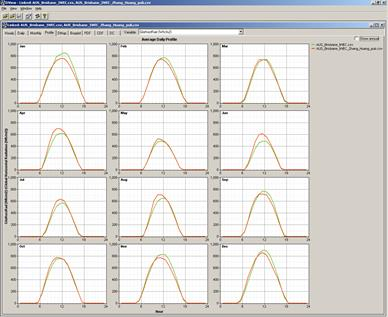
\includegraphics[width=0.9\textwidth, height=0.9\textheight, keepaspectratio=true]{media/image006.jpg}
\caption{Solar radiation comparison - IWEC vs Weather Solar Model (Brisbane AUS) \protect \label{fig:solar-radiation-comparison-iwec-vs-weather}}
\end{figure}

Of course, there are other locations that don't compare quite as well:

\begin{figure}[hbtp] % fig 11
\centering
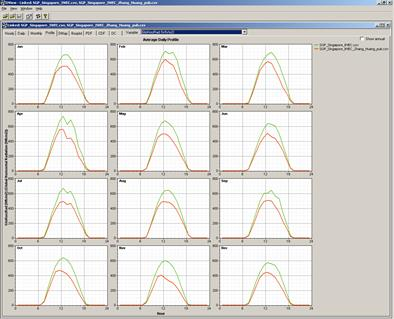
\includegraphics[width=0.9\textwidth, height=0.9\textheight, keepaspectratio=true]{media/image007.jpg}
\caption{Comparison of IWEC vs Weather program Solar Model (Singapore) \protect \label{fig:comparison-of-iwec-vs-weather-program-solar}}
\end{figure}
